\documentclass[10pt,landscape]{article}
\usepackage{multicol}
\usepackage{calc}
\usepackage{ifthen}
\usepackage[landscape]{geometry}
\usepackage{hyperref}
\usepackage{graphicx}
\usepackage{amsmath,amssymb}
\usepackage{algorithm2e}
\usepackage{float}

% To make this come out properly in landscape mode, do one of the following
% 1.
%  pdflatex latexsheet.tex
%
% 2.
%  latex latexsheet.tex
%  dvips -P pdf  -t landscape latexsheet.dvi
%  ps2pdf latexsheet.ps


% If you're reading this, be prepared for confusion.  Making this was
% a learning experience for me, and it shows.  Much of the placement
% was hacked in; if you make it better, let me know...


% 2008-04
% Changed page margin code to use the geometry package. Also added code for
% conditional page margins, depending on paper size. Thanks to Uwe Ziegenhagen
% for the suggestions.

% 2006-08
% Made changes based on suggestions from Gene Cooperman. <gene at ccs.neu.edu>


% To Do:
% \listoffigures \listoftables
% \setcounter{secnumdepth}{0}


% This sets page margins to .5 inch if using letter paper, and to 1cm
% if using A4 paper. (This probably isn't strictly necessary.)
% If using another size paper, use default 1cm margins.
\ifthenelse{\lengthtest { \paperwidth = 11in}}
	{ \geometry{top=.5in,left=.5in,right=.5in,bottom=.5in} }
	{\ifthenelse{ \lengthtest{ \paperwidth = 297mm}}
		{\geometry{top=1cm,left=1cm,right=1cm,bottom=1cm} }
		{\geometry{top=1cm,left=1cm,right=1cm,bottom=1cm} }
	}

% Turn off header and footer
\pagestyle{empty}
 

% Redefine section commands to use less space
\makeatletter
\renewcommand{\section}{\@startsection{section}{1}{0mm}%
                                {-1ex plus -.5ex minus -.2ex}%
                                {0.5ex plus .2ex}%x
                                {\normalfont\large\bfseries}}
\renewcommand{\subsection}{\@startsection{subsection}{2}{0mm}%
                                {-1explus -.5ex minus -.2ex}%
                                {0.5ex plus .2ex}%
                                {\normalfont\normalsize\bfseries}}
\renewcommand{\subsubsection}{\@startsection{subsubsection}{3}{0mm}%
                                {-1ex plus -.5ex minus -.2ex}%
                                {1ex plus .2ex}%
                                {\normalfont\small\bfseries}}
\makeatother

% Define BibTeX command
\def\BibTeX{{\rm B\kern-.05em{\sc i\kern-.025em b}\kern-.08em
    T\kern-.1667em\lower.7ex\hbox{E}\kern-.125emX}}

% Don't print section numbers
\setcounter{secnumdepth}{0}


\setlength{\parindent}{0pt}
\setlength{\parskip}{0pt plus 0.5ex}


% -----------------------------------------------------------------------

\begin{document}

\raggedright
\footnotesize
\begin{multicols}{3}


% multicol parameters
% These lengths are set only within the two main columns
%\setlength{\columnseprule}{0.25pt}
\setlength{\premulticols}{1pt}
\setlength{\postmulticols}{1pt}
\setlength{\multicolsep}{1pt}
\setlength{\columnsep}{2pt}

\begin{center}
     \Large{Reinforcement Learning Cheat Sheet} \\
\end{center}

\section{Agent-Environment Interface}
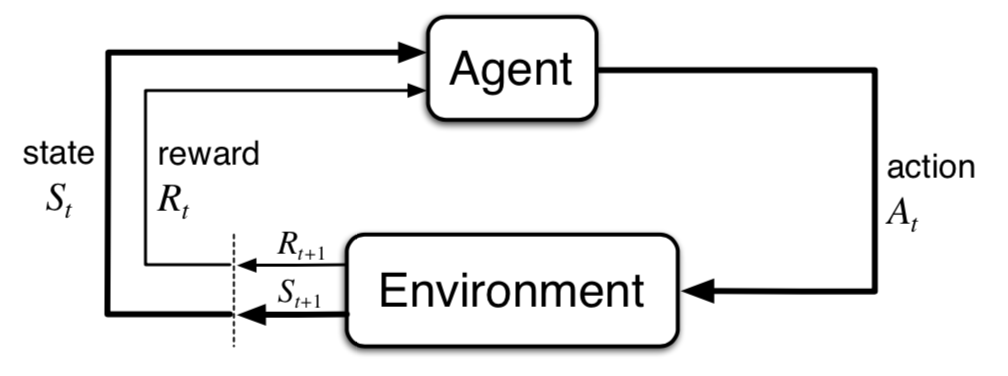
\includegraphics[width=\linewidth]{./images/Agent-Environment.png}
The Agent at each step $t$ receives a representation of the environment's \emph{state}, $S_t \in S$ and it selects an action $A_t \in A(s)$. Then, as a consequence of its action the agent receives a \emph{reward}, $R_{t + 1} \in R \in \mathbb{R}$.  

\section{Policy}
A \emph{policy} is a mapping from a state to an action
\begin{equation}
\pi_t(s|a)
\label{eq: policy}	
\end{equation}
That is the probability of select an action $A_t = a$ if $S_t = s$.

\newlength{\MyLen}
\settowidth{\MyLen}{\texttt{letterpaper}/\texttt{a4paper} \ }


\section{Reward}
The total \emph{reward} is expressed as:
\begin{equation}
G_t = \sum_{k = 0}^H = \gamma^kr_{t + k + 1}	
\label{eq: total_reward}	
\end{equation}
Where $\gamma$ is the \emph{discount factor} and $H$ is the \emph{horizon}, that can be infinite.


\subsection{Markov Decision Process}
A \textbf{Markov Decision Process}, MPD, is a 5-tuple $(S, A, P, R, \gamma)$ where:
\begin{equation}
	\begin{array}{l}
	 \text{finite set of states:} \\
	 	s \in S \\
	 \text{finite set of actions:} \\
	a \in A \\
		 \text{state transition probabilities:} \\ 	
	p(s' | s, a) = Pr \{S_{t + 1} = s' | S_t = s, A_t = a \} \\ 
		\text{expected reward for state-action-nexstate:}\\ 
	r(s',s, a) = \mathbb{E}[ R_{t + 1} | S_{t + 1} = s',  S_t = s, A_t = a ]  \\
	\end{array}
\end{equation}
\section{Value Function}
Value function describes \emph{how good} is to be in a specific state $s$ under a certain policy $\pi$. For MDP:
\begin{equation}
V_{\pi}(s) = \mathbb{E}[G_t | S_t = s)	
\label{eq: value_func}
\end{equation}

Informally, is the expected return (expected cumulative discounted reward) when starting from $s$ and following $\pi$

\subsection{Optimal}

\begin{equation}
v_*(s) = \max\limits_{\pi} v^\pi(s)
\label{eq: value_optimal}	
\end{equation}

\section{Action-Value (Q) Function}
We can also denoted the expected reward for state, action pairs.
\begin{equation}
q_{\pi}(s, a) = \mathbb{E}_{\pi}\begin{bmatrix} G_t | S_t = s, A_t = a \end{bmatrix}
\label{eq: q_func}	
\end{equation}
\subsection{Optimal}
The optimal value-action function:

\begin{equation}
q_*(s,a) = \max\limits_{\pi} q^\pi(s,a)
\label{eq: action_value_optimal}	
\end{equation}
Clearly, using this new notation we can redefine $v^*$, equation \ref{eq: value_optimal}, using $q^*(s,a)$, equation \ref{eq: action_value_optimal}:
\begin{equation}
v_*(s) = \max\limits_{a \in A(s)} q_{\pi*}(s,a)
\end{equation}
Intuitively, the above equation express the fact that the value of a state under the optimal policy \textbf{must be equal} to the expected return from the best action from that state.

\section{Bellman Equation} 
An important recursive property emerges for booth Value \ref{eq: value_func} and Q \ref{eq: q_func} functions if the expand them.
\subsection{Value Function}
\begin{equation}
\begin{array}{l l}
v_{\pi}(s) & = \mathbb{E}_{\pi}\begin{bmatrix}G_t | S_t = s\end{bmatrix} \\
\\
& =  \mathbb{E}_{\pi}\begin{bmatrix}\sum\limits_{k = 0}^{\infty} \gamma^kR_{t + k + 1} | S_t = s \end{bmatrix} \\
\\
& = \mathbb{E}_{\pi}\begin{bmatrix}R_{t + 1} + \sum\limits_{k = 0}^{\infty} \gamma^k R_{t + k + 2} | S_t = s \end{bmatrix} \\ 
\\
& = \underbrace{\sum\limits_{a} \pi(a | s) \sum\limits_{s'}\sum\limits_{r} p(s', r | s, a)}_{\text{Sum of all probabilities $\forall$ possibile $r$}} \\ 
& \begin{bmatrix} r + \gamma \underbrace{\mathbb{E}_{\pi}\begin{bmatrix} \sum\limits_{k = 0}^{\infty} \gamma^k R_{t + k + 2} | S_{t + 1} = s' \end{bmatrix}}_{\text{Expected reward from } s_{t + 1}} \end{bmatrix} \\
\\ 
& = \sum\limits_{a} \pi(a | s) \sum\limits_{s'}\sum\limits_{r} p(s', r | s, a)\begin{bmatrix} r + \gamma v_{\pi}(s')
\end{bmatrix}
\end{array}	
\label{eq: value_bellman}
\end{equation}
Similar, we can do the same for the Q function:

\begin{equation}
\begin{array}{l l}
q_{\pi}(s,a) &= \mathbb{E}_{\pi}\begin{bmatrix} G_t | S_t = s, A_t = a \end{bmatrix} \\ 
\\
&= \mathbb{E}_{\pi}\begin{bmatrix} \sum\limits_{k = 0}^{\infty}\gamma^kR_{t + k + 1} | S_t = s, A_t = a \end{bmatrix} \\
\\
&= \mathbb{E}_{\pi}\begin{bmatrix}R_{t+1} + \sum\limits_{k = 0}^{\infty}\gamma^kR_{t + k + 2} | S_t = s, A_t = a \end{bmatrix} \\
\\
&=\sum\limits_{s',r} p(s', r| s, a)\begin{bmatrix}r +\mathbb{E}_{\pi} \begin{bmatrix} \sum\limits_{k = 0}^{\infty} \gamma^k   R_{t + k + 2} | S_{t+1} = s' \end{bmatrix}  \end{bmatrix} \\
\\
 	&=\sum\limits_{s',r} p(s', r| s, a)\begin{bmatrix}r +\gamma  V_{\pi}(s') \end{bmatrix}\\
\end{array}	
\label{eq: action_value_bellman}
\end{equation}

\section{Dynamic Programming}
Taking advantages of the subproblem structure of the V and Q function we can find the optimal policy by just \emph{planning}
\subsection{Policy Iteration}
We can now, find the optimal policy 
\begin{algorithm}[H]
%\SetAlgoLined
 1. Initialisation \\
 $V(s) \in \mathbb{R}, (\text{e.g } V(s) = 0)$ and $\pi(s) \in A$  for all $s \in S$,\\
 $\Delta \leftarrow 0$ \\
 2. Policy Evaluation \\ 
 \While{$\Delta < \theta$ (a small positive number)}{
  \ForEach{$s \in S$} {
  	$v \leftarrow V(s)$\\
  	$V(s) \leftarrow \sum\limits_a \pi(a|s) \sum\limits_{s', r} p(s',r | s, a) \begin{bmatrix}
  		r + \gamma V(s')
  	\end{bmatrix}$ \\
  	$\Delta \leftarrow \max(\Delta, | v - V(s)|)$
  	}

 }
 3. Policy Improvement \\
 \emph{policy-stable} $ \leftarrow $ \emph{true} \\
 \While{not policy-stable}{
  \ForEach{$s \in S$} {
  	\emph{old-action} $\leftarrow \pi(s)$
  	$\pi(s) \leftarrow \text{argmax}\limits_a\sum\limits_{s', r} p(s',r | s, a) \begin{bmatrix}
  		r + \gamma V(s')
  	\end{bmatrix}$ \\
  	\emp{policy-stable} $\leftarrow$ \emph{old-action} $ \neq \pi(s)$  
  	  	}
 }
\caption{Policy Iteration}
\end{algorithm}

\subsection{Value Iteration}
We can avoid to wait until $V(s)$ has converged and instead to policy improvement and truncated policy evaluation step in one operation 
\begin{algorithm}[H]
%\SetAlgoLine
 \SetKwInOut{Output}{ouput}
 \SetKwInOut{Input}{inputs}
  \SetKwProg{ValueIteration}{Value Iteration}{}{}
%   \ValueIteration{$(Q,D):$}{
 Initialise $V(s) \in \mathbb{R}, \text{e.g} V(s) = 0$ \\
 $\Delta \leftarrow 0$ \\
 \While{$\Delta < \theta$ (a small positive number)}{
  \ForEach{$s \in S$} {
  	$v \leftarrow V(s)$\\
  	$V(s) \leftarrow \max\limits_a \sum\limits_{s', r} p(s',r | s, a) \begin{bmatrix}
  		r + \gamma V(s')
  	\end{bmatrix}$ \\
  	$\Delta \leftarrow \max(\Delta, | v - V(s)|)$
  	}
 }
  \Output{Deterministic policy $\pi \approx \pi_*$ such that}
  $\pi(s) = \text{argmax}\limits_a \sum\limits_{s', r} p(s',r | s, a) \begin{bmatrix}
  		r + \gamma V(s')
  	\end{bmatrix}$ 
% }
\caption{Value Iteration}
\end{algorithm} 
% }

\end{multicols}

\begin{multicols}{2}
\section{Monte Carlo Methods}
Monte Carlo (MC) is a \emph{Model Free} method, It does not require complete knowledge of the environment. It is based on \textbf{averaging sample returns} for each state-action pair. The following algorithm gives the basic implementation

\begin{algorithm}[H]
%\SetAlgoLine
 \SetKwInOut{Output}{ouput}
 \SetKwInOut{Input}{inputs}
  \SetKwProg{ValueIteration}{Value Iteration}{}{}
%   \ValueIteration{$(Q,D):$}{
 Initialise for all $s \in S, a \in A(s):$ \\
	$\quad Q(s,a) \leftarrow \text{arbitrary}$ \\  
	$\quad \pi(s) \leftarrow \text{arbitrary}$ \\  
	$\quad Returns(s,a) \leftarrow \text{empty list}$ \\  

 \While{forever}{
	\begin{enumerate}
		\item[(a)] Choose $S_0 \in S)$ and $A_0 \in A(S_0)$, all pairs have probability $ > 0$ \\
		Generate an episode starting from $S_0, A_0$ following $\pi$
		\item[(b)] For each pair $s,a$ appearing in the episode: \\ 
		$\quad G \leftarrow$ return following the first occurrence of $s,a$ \\
		$\quad$ Append $G$ to $Returns(s,a))$ \\
		$\quad Q(s,a) \leftarrow average(Returns(s,a))$ \\ 
		\item[(c)] For each $s$ in the episode: \\
		$\quad \pi(s) \leftarrow \text{argmax}\limits_a Q(s,a)$

	\end{enumerate}

 }
\caption{Monte Carlo first-visit }
\end{algorithm} 
% }
For no-stationary problems, the Monte Carlo estimate for, e.g, $V$ is:
\begin{equation}
V(S_t) \leftarrow V(S_t) + \alpha \begin{bmatrix}
	G_t - V(S_t)
\end{bmatrix}	
\end{equation}
Where $\alpha$ is the learning rate, how much we want to forget about pass experiences.
\section{Temporal Difference - Q Learning}
Temporal Difference (TD) methods learn directly from raw experience without a model of the environment's dynamics. TD substitutes the expected discounted reward $G_t$ from the episode with an estimation:
\begin{equation}
V(S_t) \leftarrow V(S_t) + \alpha \begin{bmatrix}
R_{t + 1} \gamma V(S_{t+1} - V(S_t)	
\end{bmatrix}
\end{equation}
The following algorithm gives a generic implementation.
\begin{algorithm}[H]
%\SetAlgoLine
% \SetKwInOut{Output}{ouput}
% \SetKwInOut{Input}{inputs}
%  \SetKwProg{ValueIteration}{Value Iteration}{}{}
 Initialise $Q(s,a)$ arbitrarily \\ 
  \ForEach{episode $\in$ episodes}{
 	\While{$s$ is not terminal} {
	Choose $a$ from $s$ using policy derived from $Q$ (e.g., $\epsilon$-greedy) \\
	Take action $a$, observer $r, s'$ \\ 
	$Q(s,a) \leftarrow Q(s,a) + \alpha  \begin{bmatrix}
r +  \gamma \max\limits_{a'}Q(s',a') - Q(s,a)	
\end{bmatrix}$\\
	$s \leftarrow s'$ 
	}
 }
\caption{Q Learning}
\end{algorithm}  
\section{Deep Q Learning}
Created by $DeepMind$, Deep Q Learning, DQL, substitutes the $Q$ function with a deep neural network called \emph{Q-network}. It also keep track of some observation in a $memory$ in order to use them to train the network. 
\begin{equation}
L_i(\theta_i) = \mathbb{E}_{(s, a, r, s') \sim U(D)}\begin{bmatrix}
	( \underbrace{r + \gamma \max\limits_a Q(s',a'; \theta_{i-1})}_\text{target} - \underbrace{Q(s,a;\theta_i)}_\text{prediction})^2
\end{bmatrix}
\end{equation}
Where $\theta$ are the weights of the network and $U(D)$ is the experience replay history. 

\begin{algorithm}[H]
%\SetAlgoLine
% \SetKwInOut{Output}{ouput}
% \SetKwInOut{Input}{inputs}
%  \SetKwProg{ValueIteration}{Value Iteration}{}{}
 Initialise replay memory $D$ with capacity $N$\\
 Initialise $Q(s,a)$ arbitrarily \\ 
  \ForEach{episode $\in$ episodes}{
 	\While{$s$ is not terminal} {
 	With probability $\epsilon$ select a random action $a \in A(s)$ \\
 	otherwise select $a = \max_a Q(s, a; \theta)$ \\
	Take action $a$, observer $r, s'$ \\ 
	Store transition $(s, a, r, s')$ in $D$ \\
	Sample random minibatch of transitions $(s_j, a_j, r_j, s'_j)$ from $D$ \\
	$ \text{Set } y_i \left\{ 
	\begin{array}{lll}
		r_j && \text{for terminal } s_j'\\
		r_j + \gamma \max\limits_a Q(s',a'; \theta) && \text{for non-terminal } s'_j
	\end{array}
	$ \\ 
	Perform gradient descent step on $(y_j - Q(s_j, a_j;\Theta))^2 $ \\ 
	$s \leftarrow s'$ 
	
 }}
\caption{Q Learning}
\end{algorithm}  
%---------------------------------------------------------------------------

\rule{0.3\linewidth}{0.25pt}
Copyright \copyright\ 2018 Francesco Saverio Zuppichini

\scriptsize

\href{http://wch.github.io/latexsheet/}{http://wch.github.io/latexsheet/}


\end{multicols}
\end{document}
